\documentclass[11pt]{article}

\usepackage[a4paper,margin=0.75in]{geometry}
\usepackage{amsmath,amssymb}
\usepackage{graphicx}
\usepackage{booktabs}
\usepackage{array}
\usepackage{float}
\usepackage{hyperref}
\usepackage{enumitem}
\usepackage{xcolor}
\usepackage{tikz}
\usetikzlibrary{positioning,arrows.meta,shapes.geometric}

\setlist{nosep}
\renewcommand{\arraystretch}{1.3}

\tikzset{
layer/.style={
draw,
rounded corners,
minimum width=2.2cm,
minimum height=0.9cm,
align=center,
fill=blue!10
},
arrow/.style={
-{Latex[length=3mm]},
thick
}
}

\begin{document}

%%%%%%%%%%%%%%%%%%%%%%%%%%%%%%%%%%%%%%%%%%%%%%%%%%%%%%%%%%%%

\begin{center}

{\Large\textbf{Shiv Nadar University Chennai}}

\vspace{3mm}

{\large\textbf{CS3807 -- Deep Learning Laboratory}}

\vspace{3mm}

{\Large\textbf{Experiment 4}}

\vspace{2mm}

{\Large\textbf{Comparative Study of Deep Convolutional Neural}}

{\Large\textbf{Network Architectures Using Transfer Learning}}

\end{center}

\vspace{5mm}

\begin{tabular}{|p{4cm}|p{8cm}|p{2cm}|}
\hline
Degree \& Branch &
B.Tech Artificial Intelligence \& Data Science &
Semester V\\
\hline
Subject Code \& Name &
CS3807 -- Deep Learning Laboratory &
AY: 2026--27\\
\hline
Name & R S Kirithic & \\
\hline
Register Number & 24011101082 & \\
\hline
\end{tabular}

%%%%%%%%%%%%%%%%%%%%%%%%%%%%%%%%%%%%%%%%%%%%%%%%%%%%%%%%%%%%

\section*{1. Objective}

The objectives of this experiment are

\begin{itemize}

\item Study the evolution of deep CNN architectures.

\item Compare LeNet-5, AlexNet, VGG16, GoogleNet and ResNet.

\item Understand transfer learning.

\item Fine tune pretrained CNN models.

\item Compare classification performance of different architectures.

\end{itemize}

%%%%%%%%%%%%%%%%%%%%%%%%%%%%%%%%%%%%%%%%%%%%%%%%%%%%%%%%%%%%

\section*{2. Learning Outcomes}

After completing this experiment students will be able to

\begin{enumerate}

\item Explain modern CNN architectures.

\item Differentiate LeNet, AlexNet, VGG16, GoogleNet and ResNet.

\item Implement transfer learning.

\item Fine tune pretrained CNN models.

\item Compare CNN architectures using performance metrics.

\end{enumerate}

%%%%%%%%%%%%%%%%%%%%%%%%%%%%%%%%%%%%%%%%%%%%%%%%%%%%%%%%%%%%

\section*{3. Introduction}

Deep Convolutional Neural Networks have become the dominant models for
computer vision applications because they automatically learn hierarchical
features from images. The evolution of CNNs has focused on improving
classification accuracy while reducing computational complexity and
training difficulties.

The progression of CNN architectures began with LeNet-5 and has evolved
through AlexNet, VGGNet, GoogleNet, and ResNet. Each architecture
introduced important innovations that significantly improved image
classification performance.

%%%%%%%%%%%%%%%%%%%%%%%%%%%%%%%%%%%%%%%%%%%%%%%%%%%%%%%%%%%%

\section*{4. Evolution of CNN Architectures}

\begin{center}

\begin{tabular}{|c|c|p{7cm}|}

\hline

Model & Year & Major Contribution\\

\hline

LeNet-5 & 1998 &
First practical convolutional neural network\\

\hline

AlexNet & 2012 &
ReLU activation, Dropout and GPU training\\

\hline

VGG16 & 2014 &
Uniform $3\times3$ convolution filters\\

\hline

GoogleNet & 2014 &
Inception modules for multi-scale feature extraction\\

\hline

ResNet & 2015 &
Residual learning using skip connections\\

\hline

\end{tabular}

\end{center}

%%%%%%%%%%%%%%%%%%%%%%%%%%%%%%%%%%%%%%%%%%%%%%%%%%%%%%%%%%%%

\section*{5. LeNet-5}

LeNet-5 was proposed by Yann LeCun in 1998 for handwritten digit
recognition. It consists of two convolution layers, two average pooling
layers and fully connected layers. It demonstrated that convolutional
networks could automatically learn image features without handcrafted
feature extraction.


Advantages

\begin{itemize}

\item Small number of parameters

\item Fast training

\item Suitable for OCR

\end{itemize}

%%%%%%%%%%%%%%%%%%%%%%%%%%%%%%%%%%%%%%%%%%%%%%%%%%%%%%%%%%%%

\section*{6. AlexNet}

AlexNet won the ImageNet Challenge in 2012 by reducing the
classification error significantly. It introduced ReLU activation,
Dropout regularization and GPU training.


Major innovations

\begin{itemize}

\item ReLU activation

\item Dropout

\item GPU implementation

\item Data augmentation

\end{itemize}

%%%%%%%%%%%%%%%%%%%%%%%%%%%%%%%%%%%%%%%%%%%%%%%%%%%%%%%%%%%%

\section*{7. VGG16}

VGG16 demonstrated that using multiple small $3\times3$ convolution
filters could outperform larger filters while increasing network depth.


Advantages

\begin{itemize}

\item Excellent feature extraction

\item Simple architecture

\item High classification accuracy

\end{itemize}

%%%%%%%%%%%%%%%%%%%%%%%%%%%%%%%%%%%%%%%%%%%%%%%%%%%%%%%%%%%%

\section*{8. Comparison of Architectures}

\begin{center}

\begin{tabular}{|l|c|c|c|}

\hline

Architecture &
Depth &
Parameters &
Main Contribution\\

\hline

LeNet-5 &
7 &
60K &
First CNN\\

AlexNet &
8 &
61M &
ReLU + Dropout\\

VGG16 &
16 &
138M &
Deep 3$\times3$ filters\\

GoogleNet &
22 &
6.8M &
Inception Modules\\

ResNet50 &
50 &
25.6M &
Residual Learning\\

\hline

\end{tabular}

\end{center}

\textit{These figures are the standard published parameter counts for the
original architectures on ImageNet. The versions actually trained in this
experiment are adapted for CIFAR-10's much smaller $32\times32$ images, so
their parameter counts are different -- these are reported separately in
Section 18.2.}

%%%%%%%%%%%%%%%%%%%%%%%%%%%%%%%%%%%%%%%%%%%%%%%%%%%%%%%%%%%%
\section*{9. GoogleNet (Inception Network)}

GoogleNet, proposed by Szegedy \textit{et al.} in 2014, introduced the
\textbf{Inception Module}, which performs multiple convolution operations
in parallel using different filter sizes. Instead of using only a single
kernel size, GoogleNet simultaneously applies $1\times1$, $3\times3$,
$5\times5$ convolutions and max pooling. The outputs are concatenated to
obtain multi-scale feature representations.

The use of $1\times1$ convolutions before larger kernels reduces the
number of trainable parameters and computational complexity.


Advantages

\begin{itemize}
\item Multi-scale feature extraction.
\item Fewer parameters than VGG16.
\item High computational efficiency.
\item Better classification performance.
\end{itemize}

%%%%%%%%%%%%%%%%%%%%%%%%%%%%%%%%%%%%%%%%%%%%%%%%%%%%%%%%%%%%

\section*{10. ResNet}

Increasing CNN depth often causes the \textbf{vanishing gradient problem},
making optimization difficult. ResNet solves this issue using
\textbf{skip (residual) connections}, allowing gradients to flow directly
through the network.

Instead of learning

\[
H(x)
\]

ResNet learns

\[
F(x)=H(x)-x
\]

thus,

\[
Output = F(x)+x
\]

where

\begin{itemize}
\item $F(x)$ = Residual Mapping
\item $x$ = Identity Mapping
\end{itemize}

\begin{figure}[H]
\centering

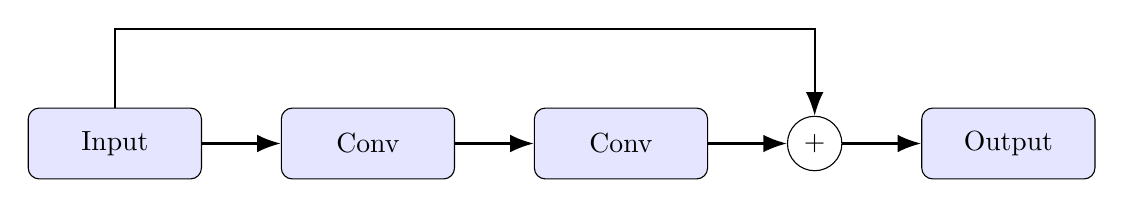
\begin{tikzpicture}[node distance=1cm]

\node[layer](input){Input};

\node[layer,right=of input](conv1){Conv};

\node[layer,right=of conv1](conv2){Conv};

\node[circle,draw,right=of conv2](add){+};

\node[layer,right=of add](output){Output};

\draw[arrow](input)--(conv1);
\draw[arrow](conv1)--(conv2);
\draw[arrow](conv2)--(add);
\draw[arrow](add)--(output);

\draw[arrow]
(input)
|-([yshift=10mm]conv2.north)
-| (add.north);

\end{tikzpicture}

\caption{Residual Block in ResNet}
\end{figure}

Advantages

\begin{itemize}
\item Eliminates vanishing gradients.
\item Enables very deep neural networks.
\item Faster convergence.
\item High ImageNet accuracy.
\end{itemize}

%%%%%%%%%%%%%%%%%%%%%%%%%%%%%%%%%%%%%%%%%%%%%%%%%%%%%%%%%%%%

\section*{11. Dilated Convolution}

Dilated convolution (also called atrous convolution) increases the
receptive field without increasing the number of parameters.

The dilation rate determines the spacing between kernel elements.

For a standard convolution,

\[
D=1
\]

For dilated convolution,

\[
D>1
\]

Example

\[
\begin{bmatrix}
1 & 0 & 2\\
0 & 3 & 0\\
4 & 0 & 5
\end{bmatrix}
\]

where zeros indicate inserted gaps.

Applications

\begin{itemize}
\item Semantic segmentation
\item Medical image analysis
\item Satellite imagery
\item Object localization
\end{itemize}

%%%%%%%%%%%%%%%%%%%%%%%%%%%%%%%%%%%%%%%%%%%%%%%%%%%%%%%%%%%%

\section*{12. Transpose Convolution}

Transpose convolution increases the spatial dimensions of feature maps.
Unlike pooling, which reduces image size, transpose convolution performs
learnable upsampling.

Applications

\begin{itemize}
\item Image Super Resolution
\item Autoencoders
\item GANs
\item Image Generation
\item Semantic Segmentation
\end{itemize}

%%%%%%%%%%%%%%%%%%%%%%%%%%%%%%%%%%%%%%%%%%%%%%%%%%%%%%%%%%%%

\section*{13. Transfer Learning}

Transfer Learning utilizes a pretrained CNN model that has already learned
general image features from a large dataset such as ImageNet.

Instead of training from scratch,

\begin{enumerate}
\item Load a pretrained model.
\item Remove the original classifier.
\item Freeze convolution layers.
\item Add new Dense layers.
\item Train the classifier.
\item Fine tune selected convolution layers.
\end{enumerate}

\begin{figure}[H]

\centering

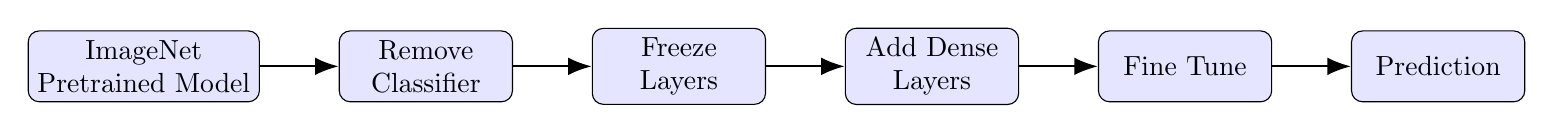
\begin{tikzpicture}[node distance=1cm]

\node[layer](a){ImageNet\\Pretrained Model};

\node[layer,right=of a](b){Remove\\Classifier};

\node[layer,right=of b](c){Freeze\\Layers};

\node[layer,right=of c](d){Add Dense\\Layers};

\node[layer,right=of d](e){Fine Tune};

\node[layer,right=of e](f){Prediction};

\foreach \x/\y in {a/b,b/c,c/d,d/e,e/f}
\draw[arrow](\x)--(\y);

\end{tikzpicture}

\caption{Transfer Learning Workflow}

\end{figure}

Advantages

\begin{itemize}
\item Faster convergence.
\item Higher accuracy on small datasets.
\item Reduced training time.
\item Lower computational cost.
\end{itemize}

%%%%%%%%%%%%%%%%%%%%%%%%%%%%%%%%%%%%%%%%%%%%%%%%%%%%%%%%%%%%

\section*{14. Dataset}

Dataset: CIFAR-10

\begin{itemize}

\item Training Images : 50,000

\item Testing Images : 10,000

\item Number of Classes : 10

\item Image Size : $32\times32\times3$

\item Classes:
Airplane, Automobile, Bird, Cat, Deer,
Dog, Frog, Horse, Ship and Truck.

\end{itemize}

The dataset was loaded directly from the pickled batch files
(\texttt{data\_batch\_1} to \texttt{data\_batch\_5} for training and
\texttt{test\_batch} for testing), stored in Google Drive, rather than
downloaded again. Each batch file unpickles to a dictionary whose
\texttt{data} field is a $10000 \times 3072$ array of pixel values and
whose \texttt{labels} field is a list of 10000 class indices, matching the
format described on the official CIFAR page. This was reshaped into
$10000 \times 32 \times 32 \times 3$ images before use.

%%%%%%%%%%%%%%%%%%%%%%%%%%%%%%%%%%%%%%%%%%%%%%%%%%%%%%%%%%%%

\section*{15. Experimental Procedure and Results}

\subsection*{Task 1: Dataset Preparation}

I loaded CIFAR-10 from the pickled batch files in Drive and normalised
the pixel values from the original $[0,255]$ range to $[0,1]$. After
normalisation, the pixel value range was confirmed to be $[0.00, 1.00]$.
The training set had 50,000 images and the test set had 10,000 images,
each $32 \times 32 \times 3$, spread across the 10 classes listed above.
One sample image from each class is shown in Figure~1.

\begin{figure}[H]
\centering
\includegraphics[width=0.85\textwidth]{figures/01_sample_images}
\caption{Sample CIFAR-10 Images (One per Class)}
\end{figure}

\textbf{Observation:} At $32 \times 32$ pixels the images are quite low
resolution, and classes that share a similar overall shape or background,
such as cat and dog, or automobile and truck, are already hard to tell
apart just by looking at them.

\subsection*{Task 2: Transfer Learning Setup}

The manual allows any one of VGG16, ResNet50, MobileNetV2 or
EfficientNetB0 for this task. I used \textbf{MobileNetV2} as the main
model for Tasks 2 to 5, since VGG16 and ResNet50 are already used
separately in the Additional Exercises (Section 20). The pretrained
ImageNet weights were loaded, the original classification layer was
removed, and the convolutional base was frozen. On top of the base I
added a Global Average Pooling layer, a Dense layer of 128 units with
ReLU activation, and a final Dense layer of 10 units with Softmax
activation.

Since CIFAR-10 images are only $32 \times 32$ and a pretrained backbone
needs a larger input to extract useful features from, images were resized
to $96 \times 96$ before being passed into the network.

The resulting model had 2,423,242 parameters in total, of which 165,258
belonged to the new head and were trainable, and 2,257,984 belonged to
the frozen MobileNetV2 base.

\subsection*{Task 3: Model Training}

The training set was split into 45,000 images for training and 5,000 for
validation. The model was compiled with the Adam optimizer at a learning
rate of 0.001, batch size 32, categorical cross-entropy loss and accuracy
as the evaluation metric, and trained for 12 epochs with the backbone
still frozen, on the Google Colab GPU runtime. This stage took 250.33
seconds. By the last epoch, training accuracy had reached 92.64\% and
validation accuracy had reached 81.24\%. Evaluated on the test set at this
point (before any fine-tuning), the model reached \textbf{80.54\%}
accuracy.

\subsection*{Task 4: Fine Tuning}

I unfroze the last 30 of the base model's 154 layers, which corresponds
to the last convolutional block, recompiled the model with a much lower
learning rate of $1\times10^{-5}$ so the pretrained weights would not be
disturbed too aggressively, and trained for 6 more epochs. Fine-tuning
took 158.69 seconds, bringing the total training time for Tasks 3 and 4
together to 409.02 seconds. By the last fine-tuning epoch, training
accuracy was 86.69\% and validation accuracy was 81.58\%. On the test
set, the fine-tuned model reached \textbf{80.26\%} accuracy, compared
with 80.54\% before fine-tuning -- a decrease of about 0.28 percentage
points.

\subsection*{Training Curves}

Figures 2 to 5 show training and validation accuracy and loss across all
18 epochs (12 frozen-training epochs followed by 6 fine-tuning epochs).

\begin{figure}[H]
\centering
\includegraphics[width=0.72\textwidth]{figures/02_training_accuracy}
\caption{Training Accuracy vs Epoch}
\end{figure}

\textbf{Observation:} Training accuracy rose steadily from 75.12\% to
92.64\% while the backbone was frozen. At the point fine-tuning began
(unfreezing the last block and dropping the learning rate), training
accuracy fell sharply to around 69.7\% before climbing back to 86.69\% by
the final epoch, without fully returning to the level it had reached
before fine-tuning.

\begin{figure}[H]
\centering
\includegraphics[width=0.72\textwidth]{figures/03_validation_accuracy}
\caption{Validation Accuracy vs Epoch}
\end{figure}

\textbf{Observation:} Validation accuracy follows a noisier version of
the same pattern, peaking near 81.86\% during the frozen stage, dropping
to about 78.9\% right after fine-tuning starts, and recovering to 81.58\%
by the last epoch -- close to, but not above, the earlier peak.

\begin{figure}[H]
\centering
\includegraphics[width=0.72\textwidth]{figures/04_training_loss}
\caption{Training Loss vs Epoch}
\end{figure}

\textbf{Observation:} Training loss decreased steadily from about 0.72 to
0.20 during frozen training, jumped back up to around 1.95 at the start
of fine-tuning, and decreased again to 0.41 by the last epoch, mirroring
the accuracy curve.

\begin{figure}[H]
\centering
\includegraphics[width=0.72\textwidth]{figures/05_validation_loss}
\caption{Validation Loss vs Epoch}
\end{figure}

\textbf{Observation:} Validation loss decreased from about 0.60 to 0.54
during frozen training, rose sharply to around 1.08 once fine-tuning
started, and settled at 0.76 by the last epoch, staying above the lowest
point reached earlier. Together, these four curves show that unfreezing
the last block and lowering the learning rate caused a real but temporary
disruption, and that six fine-tuning epochs were not quite enough to
recover past where the frozen model already was, which lines up with the
small drop in final test accuracy.

\subsection*{Task 5: Model Evaluation}

The final fine-tuned model was evaluated on the full 10,000-image test
set.

\begin{center}
\begin{tabular}{|p{6cm}|p{4cm}|}
\hline
Metric & Value\\
\hline
Testing Accuracy & 80.26\%\\
\hline
Weighted Precision & 80.28\%\\
\hline
Weighted Recall & 80.26\%\\
\hline
Weighted F1-score & 80.24\%\\
\hline
\end{tabular}
\end{center}

\begin{center}
\begin{tabular}{|l|c|c|c|c|}
\hline
Class & Precision & Recall & F1-score & Support\\
\hline
Airplane & 0.81 & 0.84 & 0.83 & 1000\\
Automobile & 0.90 & 0.91 & 0.90 & 1000\\
Bird & 0.77 & 0.74 & 0.76 & 1000\\
Cat & 0.64 & 0.65 & 0.64 & 1000\\
Deer & 0.78 & 0.76 & 0.77 & 1000\\
Dog & 0.71 & 0.70 & 0.70 & 1000\\
Frog & 0.79 & 0.86 & 0.82 & 1000\\
Horse & 0.86 & 0.81 & 0.83 & 1000\\
Ship & 0.89 & 0.86 & 0.87 & 1000\\
Truck & 0.88 & 0.90 & 0.89 & 1000\\
\hline
\textbf{Accuracy} & \multicolumn{3}{c|}{0.80} & 10000\\
\hline
Macro Avg & 0.80 & 0.80 & 0.80 & 10000\\
\hline
Weighted Avg & 0.80 & 0.80 & 0.80 & 10000\\
\hline
\end{tabular}
\end{center}

\begin{figure}[H]
\centering
\includegraphics[width=0.75\textwidth]{figures/06_confusion_matrix}
\caption{Confusion Matrix -- MobileNetV2 (Fine-Tuned)}
\end{figure}

\textbf{Observation:} The largest single confusion in the matrix is
between cat and dog: 147 cats were predicted as dog and 155 dogs were
predicted as cat, which lines up with these two classes having the lowest
recall in the table above (65\% and 70\%). Airplane and ship, and
automobile and truck, also show some mutual confusion, which makes sense
since both pairs share a similar overall shape and background.

\begin{figure}[H]
\centering
\includegraphics[width=0.85\textwidth]{figures/07_misclassified_images}
\caption{Sample Misclassified Test Images}
\end{figure}

\textbf{Observation:} The misclassified examples shown here mostly belong
to the same confusable pairs identified in the confusion matrix, and in
several cases the true and predicted classes do look genuinely similar at
this resolution.

%%%%%%%%%%%%%%%%%%%%%%%%%%%%%%%%%%%%%%%%%%%%%%%%%%%%%%%%%%%%

\section*{16. Hyperparameter Study}

Searching the full grid given in the manual (learning rate, batch size,
epochs, optimizer, dense units and frozen mode) exhaustively would mean
$2 \times 3 \times 2 \times 2 \times 2 \times 2 = 96$ combinations, which
is too many to train one by one in a lab setting. Instead, 8 combinations
were sampled at random and each was trained on a smaller stratified
subset (400 images per class for training, 100 per class for testing) so
the whole study would finish in a reasonable time. The results, ranked by
validation accuracy, are given below.

\begin{center}
\begin{tabular}{|c|c|c|c|c|c|c|}
\hline
LR & Batch & Epochs & Optimizer & Dense & Frozen & Val. Acc.\\
\hline
0.001 & 32 & 20 & Adam & 256 & All & 77.7\%\\
0.0001 & 16 & 20 & Adam & 256 & Partial & 74.3\%\\
0.0001 & 16 & 20 & SGD & 256 & All & 73.5\%\\
0.001 & 16 & 20 & Adam & 128 & Partial & 69.4\%\\
0.0001 & 32 & 10 & SGD & 128 & All & 66.2\%\\
0.0001 & 64 & 10 & SGD & 128 & All & 61.7\%\\
0.001 & 64 & 10 & Adam & 128 & Partial & 57.5\%\\
0.001 & 16 & 10 & Adam & 128 & Partial & 52.8\%\\
\hline
\end{tabular}
\end{center}

\begin{figure}[H]
\centering
\includegraphics[width=0.75\textwidth]{figures/08_hyperparameter_search}
\caption{Hyperparameter Search Results (Randomized Search)}
\end{figure}

The best combination found was a learning rate of 0.001, batch size 32,
20 epochs, the Adam optimizer, 256 dense units, and the backbone fully
frozen, reaching 77.7\% validation accuracy.

\textbf{Observation:} The number of epochs shows the clearest pattern in
this table -- all four combinations trained for 20 epochs landed in the
top four results (69.4\% to 77.7\%), while all four combinations trained
for only 10 epochs landed in the bottom four (52.8\% to 66.2\%),
regardless of the other settings. A dense layer of 256 units also tended
to do better than 128 units among the top results. Learning rate, batch
size, optimizer and whether the backbone was fully or partially frozen
did not show as clear a pattern here, which is discussed further as
Exercise 3 in Section 20.

%%%%%%%%%%%%%%%%%%%%%%%%%%%%%%%%%%%%%%%%%%%%%%%%%%%%%%%%%%%%

\section*{17. Mandatory Plots}

All of the plots required for this experiment -- sample CIFAR-10 images,
training accuracy, validation accuracy, training loss, validation loss,
the confusion matrix and a set of misclassified images -- are presented
above in Section 15, alongside the task they belong to, each with its own
brief observation.

%%%%%%%%%%%%%%%%%%%%%%%%%%%%%%%%%%%%%%%%%%%%%%%%%%%%%%%%%%%%

\section*{18. Results}

\subsection*{18.1 Performance Metrics}

\begin{center}
\begin{tabular}{|p{6cm}|p{4cm}|}
\hline
Metric & Value\\
\hline
Training Accuracy & 86.69\%\\
\hline
Testing Accuracy & 80.26\%\\
\hline
Precision & 80.28\%\\
\hline
Recall & 80.26\%\\
\hline
F1-score & 80.24\%\\
\hline
Training Time & 409.02 s\\
\hline
Total Parameters & 2,423,242\\
\hline
\end{tabular}
\end{center}

\vspace{5mm}

\subsection*{18.2 Comparison of Architectures}

This table reports what was actually measured in this experiment.
MobileNetV2 was trained on the full dataset as the main model; VGG16,
ResNet50, the AlexNet-style network and the LeNet-5-style network were
each trained on the smaller subset used for the Additional Exercises
(6,000 training images, 1,500 test images, 8 epochs). LeNet-5-style and
AlexNet-style were trained from scratch at CIFAR-10's native
$32\times32$ resolution, since no pretrained weights exist for either;
the other three used $96\times96$ resized inputs with frozen, pretrained
ImageNet weights.

\begin{center}
\begin{tabular}{|l|c|c|c|}
\hline
Model &
Parameters &
Accuracy &
Training Time (s)\\
\hline
MobileNetV2 (main, full dataset) & 2,423,242 & 80.26\% & 409.02\\
VGG16 (transfer, subset) & 14,781,642 & 63.07\% & 69.90\\
ResNet50 (transfer, subset) & 23,851,274 & 30.53\% & 50.90\\
AlexNet-style (from scratch, subset) & 6,978,890 & 44.33\% & 33.01\\
LeNet-5-style (from scratch, subset) & 83,126 & 47.60\% & 11.10\\
\hline
\end{tabular}
\end{center}

\begin{figure}[H]
\centering
\includegraphics[width=0.75\textwidth]{figures/09_architecture_comparison_accuracy}
\caption{Architecture Comparison -- Test Accuracy}
\end{figure}

\begin{figure}[H]
\centering
\includegraphics[width=0.75\textwidth]{figures/10_architecture_comparison_time}
\caption{Architecture Comparison -- Training Time}
\end{figure}

\textbf{Observation:} MobileNetV2 reached the highest accuracy by a clear
margin, but it was also trained on far more data (45,000 images against
6,000) for more epochs (18 against 8), so this is not a fair comparison
of the architectures on equal terms -- it mainly shows what the full
pipeline achieved. Among the four models trained on the same subset, VGG16
did noticeably better than ResNet50 (63.07\% against 30.53\%), even
though both used a frozen pretrained backbone with the same size input and
the same shallow head. One likely reason is that ResNet50 relies heavily
on batch normalization layers throughout its convolutional blocks, and
their statistics stay fixed once the backbone is frozen; VGG16 has no
batch normalization in its convolutional layers, so it is less sensitive
to being frozen in this way. It is also worth pointing out that the two
from-scratch networks, LeNet-5-style and AlexNet-style, both reached
higher accuracy than the frozen ResNet50 transfer-learning run on this
same subset, despite having a fraction of its parameters. This suggests
that, with only 6,000 training images and 8 epochs, training a small
network directly on CIFAR-10 worked better here than training a shallow
head on top of a frozen ResNet50 base.

%%%%%%%%%%%%%%%%%%%%%%%%%%%%%%%%%%%%%%%%%%%%%%%%%%%%%%%%%%%%

\section*{19. Discussion Questions}

\begin{enumerate}

\item \textbf{Why is AlexNet considered a breakthrough in deep learning?}
AlexNet was the first CNN to win the ImageNet competition by a large
margin, and it showed that a deep network could be trained in practice by
combining ReLU activations, which train faster than sigmoid or tanh,
Dropout to control overfitting, and GPU implementation to make training
large models feasible in a reasonable amount of time. It effectively
proved that deep learning could outperform the hand-engineered
computer-vision methods that came before it.

\item \textbf{Why does VGG16 use only $3\times3$ convolution filters?}
Stacking several $3\times3$ filters gives the same effective receptive
field as one larger filter (two $3\times3$ layers cover the same area as
one $5\times5$ layer) while using fewer parameters and adding an extra
non-linearity in between. This lets the network go deeper without the
parameter count growing as quickly as it would with larger filters.

\item \textbf{Explain the advantages of the Inception module.}
The Inception module applies several filter sizes ($1\times1$,
$3\times3$, $5\times5$) and pooling in parallel and concatenates the
results, so the network can capture features at multiple scales in the
same layer instead of having to commit to one filter size. The
$1\times1$ convolutions used before the larger filters reduce the number
of input channels first, which keeps the computational cost down even
though multiple filter sizes are being used together.

\item \textbf{What is the purpose of residual learning?}
Residual learning lets a layer learn the difference between its input and
its desired output, $F(x) = H(x) - x$, instead of learning the full
mapping $H(x)$ directly. The skip connection then adds the input back,
$F(x) + x$, which gives the gradient a direct path back through the
network during backpropagation. This makes very deep networks much
easier to optimize, since it avoids the vanishing gradient problem that
made earlier deep networks hard to train.

\item \textbf{Differentiate LeNet and ResNet.}
LeNet-5 is a shallow network with about 60 thousand parameters, built
from two convolution layers and two average pooling layers, and designed
for small greyscale digit images. ResNet50 is a much deeper network with
around 25.6 million parameters, and its main innovation, residual skip
connections, is exactly what makes that extra depth possible to train in
the first place. In this experiment, the LeNet-5-style network trained
here had 83,126 parameters, in the same range as the original, while the
transfer-learning ResNet50 run kept its much larger frozen backbone.

\item \textbf{What is Transfer Learning?}
Transfer learning means reusing a model that has already been trained on
a large dataset, usually ImageNet, as the starting point for a new,
usually smaller, task, instead of training a new network from scratch.
The convolutional base is generally kept frozen so its learned features
are reused directly, and only a new classification head is trained on the
new dataset.

\item \textbf{Why is fine tuning required?}
Features learned from ImageNet are general, but they are not perfectly
suited to a different dataset such as CIFAR-10. Fine-tuning unfreezes some
of the later layers of the base network, which tend to hold more
task-specific features, and retrains them at a low learning rate so they
can adjust slightly to the new dataset, on top of the new classification
head that was already trained. In this experiment fine-tuning did not
improve test accuracy (it went from 80.54\% to 80.26\%), which shows that
fine-tuning is not guaranteed to help within a small number of epochs --
if the learning rate or the number of unfrozen layers is not well suited
to the new data, it can disturb the pretrained features before the model
has time to settle back down.

\item \textbf{Explain the difference between dilated convolution and
transpose convolution.}
Dilated convolution keeps the output the same size as a normal
convolution but spreads the kernel elements further apart, which
increases the receptive field without increasing the number of
parameters; it is mainly used to gather more context, for example in
semantic segmentation. Transpose convolution does the opposite job: it
increases the spatial size of the feature map, effectively learning how
to upsample, and is mainly used to reconstruct or generate images, for
example in autoencoders or generative networks.

\item \textbf{Why do pretrained models converge faster?}
A pretrained model already has convolutional filters tuned to detect
general features such as edges, textures and shapes, learned from a very
large dataset. Starting from these weights instead of random
initialisation means the network does not have to relearn these basic
features from nothing, so fewer epochs are needed for it to reach a
reasonable accuracy on the new task.

\item \textbf{Compare the computational complexity of LeNet and ResNet.}
LeNet-5 is computationally light, with roughly 60 thousand parameters and
only two convolution layers, so it trains quickly even on a CPU. ResNet50
is far heavier, with around 25.6 million parameters across 50 layers, and
normally needs a GPU to train in a reasonable time. This difference shows
up directly in this experiment: the LeNet-5-style network trained in
11.10 seconds on the subset, compared with 50.90 seconds for the ResNet50
transfer-learning run on the same subset.

\end{enumerate}

%%%%%%%%%%%%%%%%%%%%%%%%%%%%%%%%%%%%%%%%%%%%%%%%%%%%%%%%%%%%

\section*{20. Additional Exercises}

\subsection*{Exercise 1: Transfer Learning Using VGG16}

VGG16 was set up the same way as the main MobileNetV2 model -- pretrained
ImageNet weights, frozen convolutional base, Global Average Pooling
followed by a Dense head -- and trained on the smaller subset (6,000
training images, 1,500 test images) for 8 epochs. It reached
\textbf{63.07\%} test accuracy, with 14,781,642 total parameters, and
took 69.90 seconds to train.

\subsection*{Exercise 2: Transfer Learning Using ResNet50}

ResNet50 was set up and trained the same way, on the same subset. It
reached \textbf{30.53\%} test accuracy, with 23,851,274 total parameters,
and took 50.90 seconds to train -- noticeably lower accuracy than VGG16
under the same conditions, discussed further in Section 18.2.

\subsection*{Exercise 3: Adam vs SGD}

This comparison is drawn from the Section 16 hyperparameter search, which
already varies the optimizer across its sampled combinations.

\begin{center}
\begin{tabular}{|l|c|c|c|}
\hline
Optimizer & Mean Val. Accuracy & Best Val. Accuracy & Combinations Sampled\\
\hline
Adam & 66.34\% & 77.7\% & 5\\
SGD & 67.13\% & 73.5\% & 3\\
\hline
\end{tabular}
\end{center}

\begin{figure}[H]
\centering
\includegraphics[width=0.55\textwidth]{figures/11_adam_vs_sgd}
\caption{Adam vs SGD (Section 16 Search Results)}
\end{figure}

\textbf{Observation:} Across the 8 randomly sampled combinations, Adam
and SGD ended up with a similar mean validation accuracy (66.34\% against
67.13\%), and the single best result overall came from Adam (77.7\%).
Since only 8 combinations were sampled in total and the other
hyperparameters were not held fixed between them, this is not a
controlled comparison of the two optimizers on their own -- it mainly
shows that neither optimizer was clearly better across the settings that
happened to be sampled.

\subsection*{Exercise 4: Frozen Layers vs Fine-Tuning}

This reuses the Task 3 and Task 4 results for the main MobileNetV2 model.

\begin{center}
\begin{tabular}{|l|c|}
\hline
Configuration & Test Accuracy\\
\hline
Frozen backbone only (Task 3) & 80.54\%\\
Fine-tuned, last block unfrozen (Task 4) & 80.26\%\\
\hline
\end{tabular}
\end{center}

\begin{figure}[H]
\centering
\includegraphics[width=0.6\textwidth]{figures/12_frozen_vs_finetuned}
\caption{Frozen vs Fine-Tuned (MobileNetV2)}
\end{figure}

\textbf{Observation:} Fine-tuning the last block did not improve test
accuracy here; it went down slightly, by 0.28 percentage points. As shown
by the training curves in Section 15, unfreezing those layers caused
training and validation accuracy to drop sharply before recovering, and
six fine-tuning epochs were not enough for the model to fully return to,
let alone exceed, where it already was with the backbone frozen.

\subsection*{Exercise 5: Precision, Recall and F1-score}

This reuses the Task 5 evaluation of the final fine-tuned MobileNetV2
model: weighted precision of 80.28\%, weighted recall of 80.26\%, and
weighted F1-score of 80.24\%. The full per-class breakdown is given in
the classification report table in Section 15.

\subsection*{Exercise 6: LeNet-5 vs AlexNet-Style vs ResNet50}

Since neither LeNet-5 nor AlexNet has pretrained weights available in
standard deep learning libraries, and neither's original design matches
CIFAR-10's resolution (AlexNet expects $227\times227$ images, and
LeNet-5 was designed for single-channel $32\times32$ digit images), both
were implemented here as their usual CIFAR-10 adaptations and trained
from scratch: LeNet-5-style kept the original two-convolution,
two-average-pool, three-fully-connected structure, and AlexNet-style kept
the five-convolution-block structure but with smaller kernels sized for
$32\times32$ inputs. Both were trained on the same subset as ResNet50
(6,000 training images, 1,500 test images, 8 epochs).

\begin{center}
\begin{tabular}{|l|c|c|c|}
\hline
Model & Parameters & Accuracy & Training Time (s)\\
\hline
LeNet-5-style (from scratch) & 83,126 & 47.60\% & 11.10\\
AlexNet-style (from scratch) & 6,978,890 & 44.33\% & 33.01\\
ResNet50 (transfer learning) & 23,851,274 & 30.53\% & 50.90\\
\hline
\end{tabular}
\end{center}

\textbf{Observation:} Both from-scratch networks reached higher accuracy
than the frozen ResNet50 transfer-learning run on this subset, and
LeNet-5-style did so with a fraction of a percent of ResNet50's parameter
count. This lines up with the observation already made in Section 18.2:
with only 6,000 training images and 8 epochs, a small network trained
directly on the data ended up more effective here than a much larger
pretrained network with only its head trainable.

%%%%%%%%%%%%%%%%%%%%%%%%%%%%%%%%%%%%%%%%%%%%%%%%%%%%%%%%%%%%

\section*{21. References}

\begin{enumerate}

\item Yann LeCun, Leon Bottou, Yoshua Bengio and Patrick Haffner,
\emph{Gradient-Based Learning Applied to Document Recognition},
Proceedings of the IEEE, 1998.

\item Alex Krizhevsky, Ilya Sutskever and Geoffrey Hinton,
\emph{ImageNet Classification with Deep Convolutional Neural Networks},
NeurIPS, 2012.

\item Karen Simonyan and Andrew Zisserman,
\emph{Very Deep Convolutional Networks for Large-Scale Image Recognition},
ICLR, 2015.

\item Christian Szegedy et al.,
\emph{Going Deeper with Convolutions},
CVPR, 2015.

\item Kaiming He, Xiangyu Zhang, Shaoqing Ren and Jian Sun,
\emph{Deep Residual Learning for Image Recognition},
CVPR, 2016.

\item Ian Goodfellow, Yoshua Bengio and Aaron Courville,
\emph{Deep Learning},
MIT Press, 2016.

\item TensorFlow Documentation:
\url{https://www.tensorflow.org}

\item Keras Documentation:
\url{https://keras.io}

\item Alex Krizhevsky, \emph{Learning Multiple Layers of Features from
Tiny Images} (CIFAR-10/CIFAR-100 dataset description):
\url{https://www.cs.toronto.edu/~kriz/cifar.html}

\end{enumerate}

%%%%%%%%%%%%%%%%%%%%%%%%%%%%%%%%%%%%%%%%%%%%%%%%%%%%%%%%%%%%

\end{document}
